
\chapter{An overview of \rtd\ Code Generator and \ee}

\label{cha:overview}

\rtd\ is an open and extensible environment, based on XML and open
standards (Java) allowing generation of portable OSEK C code from OIL
definitions to create applications that run in real-time in a variety
of environments, including dsPIC, AVR, ARM7, Altera Nios II, and
others.

Generated code can run on any OSEK-compliant system, but the \rtd\
framework is optimized for running in conjunction with the \ee\ 
%OSEK
kernel.

%\rtd\ lets you speed up the coding process. Figure \ref{fig:rtd}
%illustrates the role of the \rtd\ (shaded elements) componentsin the
%software design process.
%
%
%\begin{figure}
%\nb{Peppe: Questa figura manca...}
%
%\caption{Application development with \rtd\ and \ee.}
%
%\label{fig:rtd}architecture\}
%\end{figure}


Because of its generic framework, the \rtd\ give a extensible modeling
and analysis platform for modeling any hardware and software,
providing compatibility with most of the model-based methodologies for
functional design on the market. The tool is designed aiming at the
following general goals:

\begin{description}
\item [Modularity:]once the kernel module is installed, each design
activity in the development flow is in charge of a module that can be
separately purchased and used as standalone component.
\item [Portability~across~different~execution~environments:]the tool
is designed and implemented in Java for maximum portability to
different environments and operating systems (MS Windows 2000/Xp,
Linux, Macintosh).
\item [Extensibility:]future extensions include custom plug-ins and
integration with third party production tools for code generation
complying with industrial standards: such as the OSEK and its related
standards (OIL, ORTI) in the automotive domain. In particuler, future
enhancements include:

\begin{itemize}
\item Graphic interface for placement and configuration options 
\item Support for the ORTI standard for debugging 
\item Support for the Lauterbach tools, for tracing and measurement of
  time-related attributes.
\end{itemize}
\end{description}


\section{Software design with \rtd{}}
%
%\nb{TBD: Early draft, showing connections with the other tools in the
%\rtd\ family}
%
%

The architecture of the \rtd\ family of tools is shown in Figure
\ref{fig:rtdruid-plugin-architecture}. Model information (i.e. for
both the functional and the architecture-level components) is stored
in an internal repository and it is made available by means of an open
format based on XML.

The toolset architecture is based on a kernel, or Core module, providing
management of internal data structure and basic services for GUI and
additional plugin modules.

Plugins exploit kernel services in order to provide support to the
design stages in a completely independent way. Here is a list of the
plugins currently available:

\begin{itemize}
\item \rtd\ Modeler;
\item \rtd\ Schedulability Analyzer;
\item \rtd\ Code generator for multiprocessors (including extensions
  for Altera programmable HW);
\end{itemize}
Future extensions include

\begin{itemize}
\item Trace viewer/Analyzer;
\item Scheduling Simulator;
\item Importers from Mathworks Simulink, ASCET and UML 2.0 models.
\end{itemize}
%
\begin{figure}
\begin{center}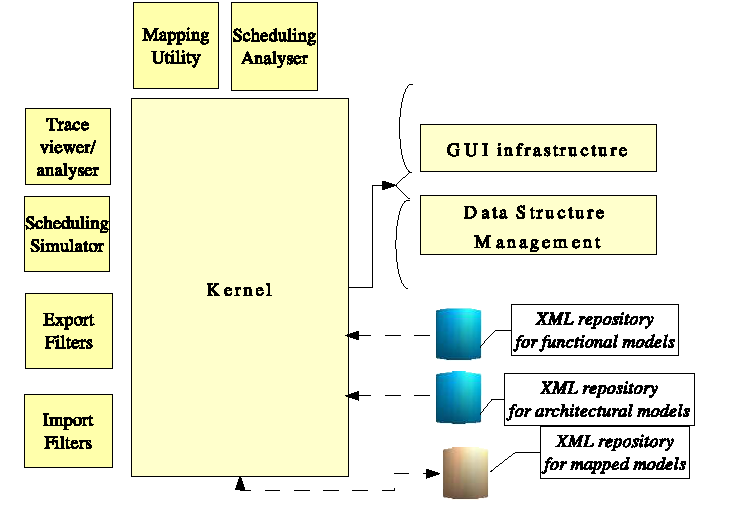
\includegraphics[%
  scale=0.7,bb=0 0 736 529]{images/rtd_plugin_arch.png}\end{center}
\caption{\label{fig:rtdruid-plugin-architecture}The plug-in architecture of \rtd.}
\end{figure}



\section{The open architecture of the \rtd\ tool}

%

\rtd\ allows saving all system information in an open XML
format. Information about the system model, configuration information
and the result of operations performed by plug-in tools, such as
schedulability analysis, tracing or debugging info, can easily be made
available to external or third party tools. Similarly, OIL files can
be imported from or exported to third party products.


\section{\rtd\ integration with Eclipse}

\rtd\ is entirely written in Java. It is based on well-known
development frameworks such as Eclipse, the framework originally
propoted by IBM and now released as an open source development
environment \cite{Eclipse}, and on the W3C XML standard. The \rtd\ tool
%
% /toOl: spendiamo due parole per dettagliare le seguenti sigle?
%
makes use of several Eclipse plug-ins, including EMF
\cite{Eclipse-EMF}, GEF \cite{Eclipse-GEF} and CDT
\cite{Eclipse-CDT}\footnote{CDT is the Eclipse component in charge of
C/C++ project management.}.

The integration of \rtd\ with the Eclipse framework easily allows any
user to perform the operations of editing, compiling, debugging and
running the software. The required commands and action sequences are
those common to all Eclipse projects, including CDT.

Similarly, operation for creating a new project, as shown in the
following Chapter \ref{cha:creating-rtdruid-project} and editing of
the configuration files follow the standard Eclipse pattern. The
result of the generation of the configuration file by the \rtd\ wizard
and the result of most operations performed by \rtd\ are shown in a
dedicated Eclipse console (as happens for most Eclipse plug-ins, for
details, please see Section \ref{cha:code-generation}).

Integration with Eclipse is not only at GUI interface level, but it 
also allows performing operations in batch (command
line) mode according to the ANT standard \cite{ANT}. \rtd\ extends the
ANT commands (``TASK'' in ANT terminology) adding the capability for
code generation and the execution of the compilation scripts starting
from an OIL file.


\section{Multiprocessor Version}

\rtd\ provides special support for the development of multiprocessor
applications together with the \ee\ kernel. Currently
supported features include:

\begin{itemize}
\item Multiprocessor systems with shared memory.
\item Support for code placement in a multiprocessor system.
\end{itemize}

Programming-level implementation is independent from code placement on
processors, meaning that the programmer do not need to be aware of the
existence of multiple processors. The code generator provides the
correct implementation of system primitives based on the placement of
the threads and resources as specified in the \rtd\ (OIL)
configuration part. Independence from placement options provides:

\begin{itemize}
\item Easy testing of different placement configurations. 
\item Easy extension to a higher degree of parallelism and seamless
  porting of existing single processor applications
\end{itemize}

\section{Multiprocessor extensions for Altera Nios II (Target specific info)}

The multiprocessor extensions allow for processor specific features
including compatibility with multicore targets like Altera Nios II,
allowing reuse of standard Altera peripherals and device
drivers. Integration with Altera's development tools, including Nios
II IDE is also supported: basically, Eclipse CDT is extended by
\rtd\ in order to allow creation and manegement of projects for
multiprocessor systems based on \ee{}.

\subsection{Integration with Nios II IDE}

The required commands and action sequences for editing, compiling,
debugging and running code produced in the \rtd\ framework are
identical to those common to Nios II IDE projects. 
%However, GEF is not
%available in the version for Altera's processors.  \nb{PJ: cosa vuol
%dire che GEF non � disponibile?}

Integration with the Nios II IDE is not yet fully automated. In the
description of the system, \rtd\ requires information related to the
HW architecture running the system, such as the number of available
CPUs and the available RAM addresses. In the current version, this
information needs to be provided by the user by writing suitable
entries inside the configuration file, and it needs to be consistent
with the definitions provided inside Altera's SOPCbuilder.

The compilation stage, however, offers full integration with the Nios
II IDE environment. The compilation stage is handled by Eclipse, and
in particular by CDT, starting from the scripts generated by \rtd\,
which, in turn, exploits the compilation environment made available by
Altera Nios II IDE. The end-result is a sequence of steps identical to
those performed when commanding from the Eclipse interface the
compilation of a standard Nios II IDE project, with the only
difference that an \rtd\ project allows handling code distributed
among multiple processors, whereas standard, automatically handled
Nios II IDE projects assume deployment of a project for each CPU.

\section{Code generation}

The \rtd\ Code Generator is a plugin that is used to automatically
generate configuration code at compile time. The steps performed by
the Code Generator upon a compilation request are described in this 
section.

\paragraph{Creation of the build directory and its content}
Starting from an OIL configuration file, the tool creates a directory
that will contain all the generated files\footnote{For Altera Nios II
users: That directory has the same meaning of those created by Altera
Nios II IDE projects for the parameter configurations, like
\file{Debug}, \file{Release}, and so on.}. The directory will be the
default directory for all the operations of the C/C++ compiler. In the
following, we assume that the name selected for this directory in the
configuration file is \file{Debug}.

The first file that is created is the \file{makefile}, created inside
the \file{Debug} directory itself. The \file{makefile} is used to
compile the application source code. The makefile structure may depend
on the final target architecture.

On a multicore system, the makefile is responsible of triggering the
compilation of a separate image for each CPU. In that case, together
with the \file{makefile}, the tool also generates a file
\file{common.mk} (inside the \file{Debug} directory), containing
common makefile settings for the CPUs in the project.

\paragraph{Creation of the CPU build directories.}
Following the creation  of the project main directory,  the \rtd\ Code
Generator  creates a  directory for  each CPU  inside the  it.  If the
system for which  the project is compiled is  a single-processor, only
one folder is created. The name of the cpu folders follows the name/ID
definitions  provided  in  the  OIL  file  for the  CPUs\footnote{CPU
names/IDs {\bf must not} contain spacing characters}.

All CPU folders contain the same files, with the exception of the
folder for the Master CPU\footnote{For informations about the Master
CPU, please refer to Section \ref{sub:master-cpu}}, which
contains the extra file \file{common.c}, containing information common
to all the CPUs in the system. In the examples shipped with \ee\,
\const{cpu0} is the predefined ID for the Master CPU.

For each CPU the Code generator produces the following files (see
Figure \ref{rtdruid-project-folders}):
\begin{description}
%
%PJ: perch� non posso mettere \file{eecfg.h}?
%
\item[{\tt eecfg.h}.] This file contains the declarations of all the
  RTOS symbols (tasks, resources, alarms, events, and so on) that are
  visible from the given CPU. The objects visible from a CPU are the
  objects allocated on it, plus the objects on other CPUs that may be
  referred by the code running on the CPU itself.

\item[{\tt eecfg.c}.] This file contains the configuration data structures of
  the \ee\ kernel, providing information on the options of the local objects
  defined in the OIL file.

\item[{\tt cpu.mk}.] This file contains the rules used to compile the
  source code allocated to the CPU.  Together with the
  \file{common.mk} file it provides information equivalent to the
  contents of the \file{makefile} created by the Nios II IDE C/C++
  Application Projects.

\item[{\tt subdir.mk}.] This file contains the list of the files that
  must be compiled and linked in order to generate the executable to
  be run on the CPU. The files depend on the partitioning
  configuration defined in the OIL file.
  \begin{warning}
    To be included inside \file{subdir.mk}, a file needs to be listed
    inside the OIL declaration. The behavior is different from normal
    Altera Nios II Projects where the fact that a file is inserted in
    a project implies that it will be automatically added to the
    \file{subdir.mk} and compiled.
  \end{warning}
\end{description}

\begin{figure}
\begin{center}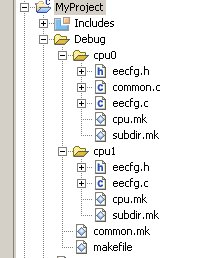
\includegraphics[%
  scale=0.8, bb=0 0 211 258]{images/rtd_project_folders.png}\end{center}
\caption{\label{rtdruid-project-folders} Folders and files created by
\rtd\ for an Altera Nios II multicore design.}
\end{figure}


%\section{ERIKA: an RTOS for predictable real-time applications}

%\nb{TBD}

